\documentclass[12pt]{scrartcl}

\usepackage{fullpage}
\usepackage{graphicx}

\title{Honors Thesis}
\author{Gina Chun}


\begin{document}

\maketitle

\newpage

\begin{abstract}
  Abstract...
\end{abstract}

\newpage

\tableofcontents

\newpage

\section{Introduction}\label{Introduction}



\subsection{why carbon is important}\label{Test}

% In this section to say blah

Carbon is one of the most important and widely investigated
elements. Carbon is all around us in a variety of forms and is an area
of study which has huge significance across many scientific fields and
applications. Carbon is in living organisms and is essential for
living organisms, thus the study of carbon would further develop the
complex workings of the environment, ecosystems and the carbon
cycle. It would also help the understanding of fossil fuels, aid the
challenges of energy-related issues, and work towards solutions for
climate change. Carbon materials are also intertwined in modern
economic industries such as in steel, clothing, pigment, plastic and
synthetic materials, and in electrodes and other similar electricity
conducting machinery. Studying carbon allows for further advancement
in these important industries which would lead to better and more
easily accessible devices, tools, and products for general society.

Now referencing the introduction \ref{Test}

\subsection{why use machine learning}
As carbon is an important element, its versatility makes it a very
complex subject of study. Carbon manifests in various physical forms,
called allotropes, each with very different properties. Because of
this, studying carbon can be difficult with conventional
methods. Using Gaussian Approximation Potentials (GAP), machine
learning can be much more cost and time efficient than traditional
scientific methods of experimentation. Machine learning also opens up
a new space of empirical methods for experiments that scientists
cannot physically replicate with traditional techniques. For example,
machine learning can be used for experiments in very small spatial
scales or for large scale simulations all while maintaining high
performance accuracy.

Here is an example of a citation: \cite{gap20}, \cite{DGL}

\newpage

\section{Background}

\begin{figure}
  \centering
  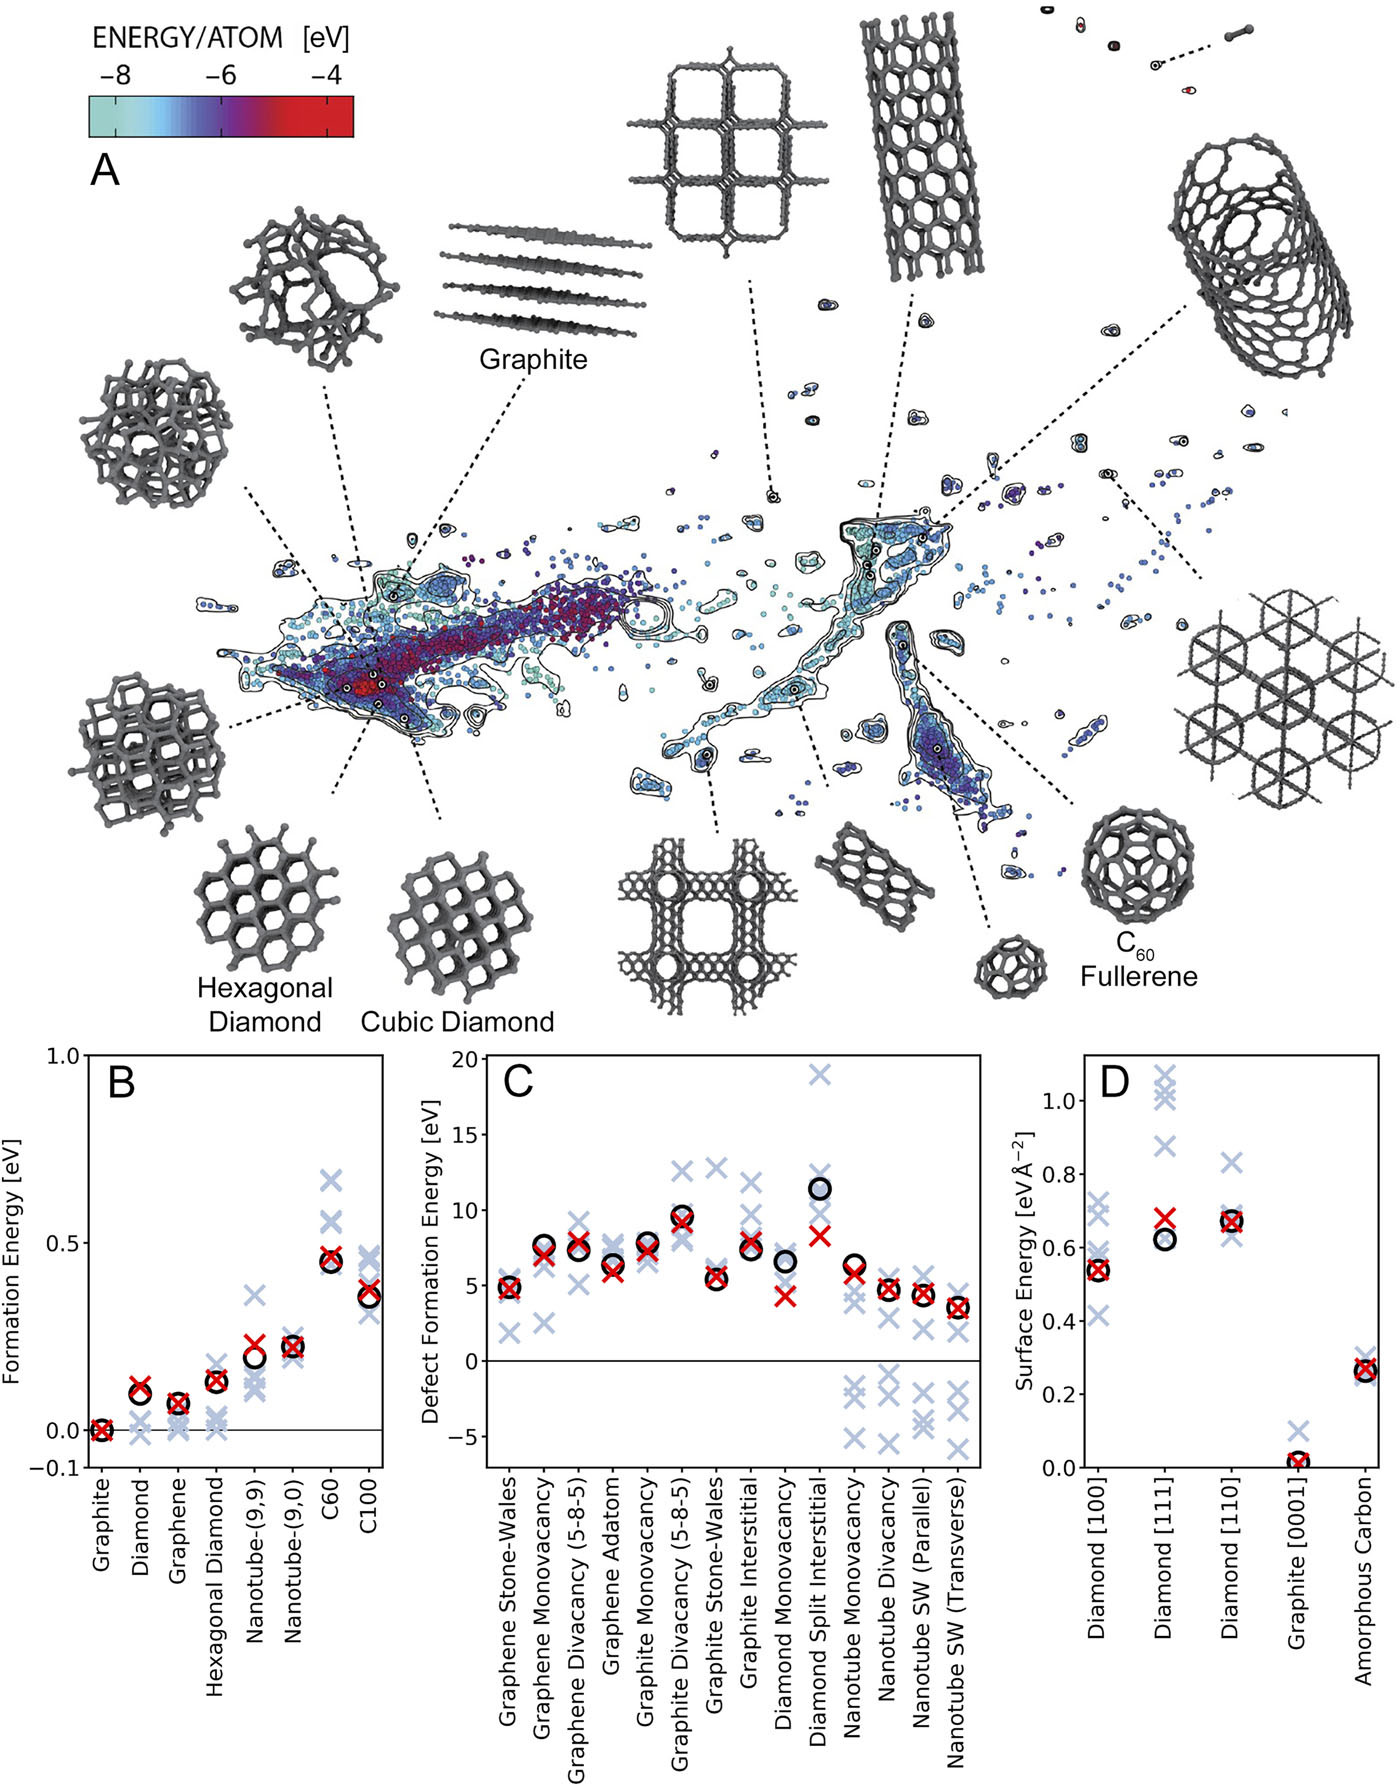
\includegraphics[scale=2]{carbon}
  
  \caption{Nice caption}\label{fig:my_figure}
\end{figure}

In figure \ref{fig:my_figure}

Graph neural networks (message passing)

Quantum chemistry

\newpage 

\section{Method}

\newpage

\section{Experimental Evaluation}

Describe experiments precisely, report results, analysus results

\newpage

\section{Conclusion}

\newpage

\bibliographystyle{plain}
\bibliography{ref}


\end{document}
